\section{Future Work}
\label{sec:conclusions:future}
In this dissertation, by utilizing structural inductive biases and natural language as inductive biases, we designed effient deep linguistic structured prediction methods with indepdent factorization. Though these methods achieved better performance on various broad-coverage and application-specific symbolic representations, there is still room for further improvment. In this section, we demonstrate the future directions including extending to other kinds of factorizations beyond independent factorization~(\autoref{ssec:future:other-factorization}), applying to other symbolic representations~(\autoref{ssec:future:other-application}), enhancing contextualized representation~(\autoref{ssec:future:contextual-rep}), repressenting other kind of biases~(\autoref{ssec:future:other-biases}), and more ways of learning and transferring the inductive biaes~(\autoref{ssec:future:bias-learn-transfer})

\subsection{Beyond Independent Factorization}
\label{ssec:future:other-factorization}

This dissertation mainly focuses on independent factorization, which ignores
the interdependence between output parts. Our experiments show that
the contextualized representation can capture the interdependence
within the input parts; thus, they can offer discriminative features
to predict each output part independently. However, we also can extend
our work on other factorizations such as \kw{auto-regressive
  factorization}, or arbitrary high order factorizations. In those
cases, the output parts will either depend on the previously predicted
output or have other high order dependecies. Take the auto-regressive
factorization as an example, we consider a more broad-coverage
construction of output \OUT~as sequential decisions as shown
in~\autoref{eq:auto-factor}.
\begin{equation}
  \label{eq:auto-factor}
E(x, y)=\sum_{j=0}^{M}E(y_{j}|x,y_{<j})
\end{equation}
In autoregressive factorization, as shown in
~\autoref{fig:autoreg-example}, for every step, a new decision $y_{j}$
will depend on the input $x$ and previous decisions $y_{<j}$. In this
case, the main challenge of the model is to learn the representation
of $x$ and previous sequential decisions $y_{<j}$, then make a
decision $y_{j}$ based on them.  Especially inspired by distributed
representation of the natural language, we also study the distributed
representation of the output structures $y_{<j}$, and leverage them to
guide constrained structured prediction.

\begin{figure}[h]
\centering
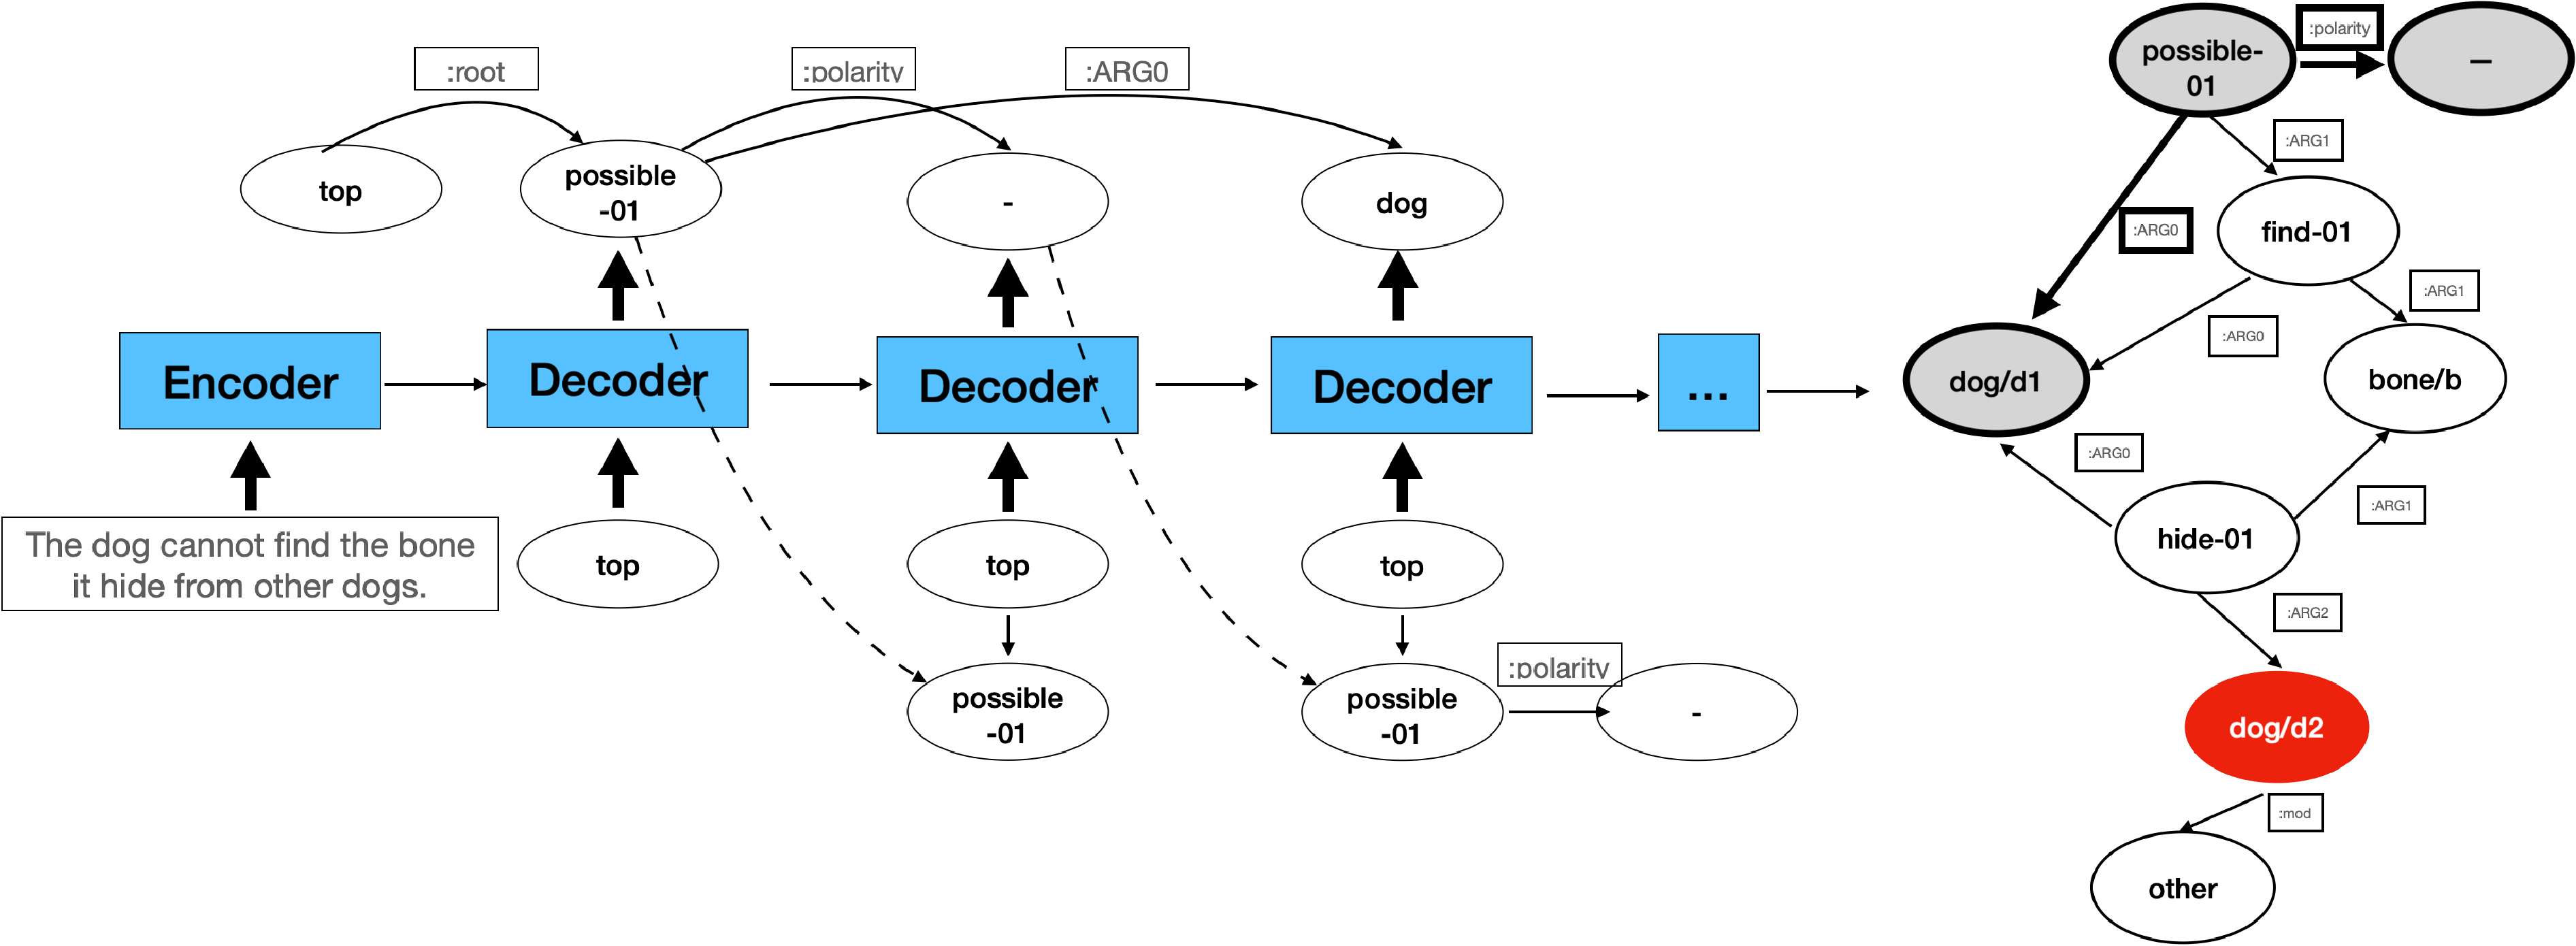
\includegraphics[width=0.92\textwidth]{seq2graph.pdf}
\caption{\label{fig:autoreg-example}The autoregressive factorization
  of AMR Parsing in different decoding time step.}
\end{figure}

\subsection{Apply to Other Symbolic Representations}
\label{ssec:future:other-application}

As shown in~\autoref{chap:lexical-phrasal}, the above structural
inductive bias in lexical, phrasal, and sentential anchoring can be
easily extended to other linguistic structured prediction tasks, such
as coreference resolution, semantic role labeling, where the main task
structures has been studied in our broad-coverage meaning
representation parsing. Taking the \kw{coreference resolution} tasks
as an example, we show how to apply the independent factorization on a
new task in~\autoref{sssec:future:coref}. Then we show the potential
future application on other symbolic representations
in~\autoref{sssec:future:other-tasks}.

\subsubsection[Coreference Resolution]{Coreference Resolution}
\label{sssec:future:coref}
 Coreference resolution is the task of clustering mentions in
text that refer to the same underlying real-world entities or
events. As shown in the left bottom of \autoref{fig:intro:dog-amr},
``dog" and ``it" are pointed to the same dog.

First, we consider the \textbf{output decomposition} for coreference
resolution task.  A classic problem formula for coreference resolution
task is to define a set of antecedent assignments $y_{i}$ for each of
span $x_{i}$ in the given document. The set of possible assignments
for each $y_{i} \in {\Phi, 1,...i-1}$. $\Phi$ means dummy antecent or the span
$i$ is not a mention, and every $y_{i}$ can be assigned with the
preceding spans.  Hence, then there are three factors for the
pair-wise coreference core.
\begin{inparaenum}[(1)]
\item predict $I_{m}(i)$, whether span $i$ is a mention.
\item predict $I_{m}(j)$, whether span $j$ is a mention.
\item search for $y_{i}$, based on the previous mention predictions
  $I_{m}(i)$ and $I_{m}(j)$.
\end{inparaenum}
One problem with the above factorization is that the third factor
$y_{i}$ may have multiple values, which are antecedent for multiple
preceding spans. Furthermore, it is not easy to do $N$ ways
classification directly, because for each $y_{i}$ the output candidate
labels are different, and the features only from span $i$ may not
enough to produce the $y_{i}$. Instead, a better independence
factorization can model this into a two-stage pipeline model as shown
in AMR parsing: Stage 1, predicting the possible mentions via local
classifier for each local factor $I_{m}(i)$. Stage 2, predicting the
edges labels between all pairs as local binary classification
$I_{a}(i,j)$, which means whether span $i$ and $j$ are in the same
cluster without caring about the preceding or not. In this output
factorization, we can model two part of contextualized representation
from span $i$ and span $j$. Such a pair-wise factorization will offer
more discriminative features and simplifer all the classification into
binary classification.  We still can use a biaffine classifier to
model the pair-wise binary classification. Furthermore, logic
constraints can be added here to enforce the consistency between local
decisions.

Then, we consider the \textbf{input decomposition and alignment
  discovery} for coreference resolution. According to the above
analysis on output decomposition, we need to decompose the inputs into
candidate spans. Assuming there are $N$ words in the input document,
then there will be~$\frac{T(T+1)}{2}$ possible spans. However, we
don't need to consider the spans cross the sentence boundaries, and we
only mainly consider the pronouns, nouns , and other entity-related or
event-related spans. Hence, such inductive biases about extracting
potential spans will also simplify the input decomposition. At the
same time, the pruning of the spans will reduce the computation for
the second stage on binary edge label prediction.

Hence, our proposed methods for two-stage graph-based parsing can be
used in coreference resolution with task-specific output
decompositions and input decompositions. The contextualized
representation for each span can also benefit from span representation
we studied in phrasal-anchoring parsing~\autoref{ssec:phr:span}

\subsubsection{Independent Factorization for Other Tasks}
\label{sssec:future:other-tasks}

For broad-coverage symbolic representations, our dissertation only
covers the representation for a single sentence. While in the future,
we also study on multisentence and document-level representations
such as MS-AMR~\cite{ogorman-etal-2018-amr},
Doc-AMR~\cite{naseem-etal-2022-docamr}, discourse
parsing~\cite{carlson-etal-2001-building}, and soon on.

For application-specific symbolic representations, besides the single
sentence representation
in~\cite[TOP,][]{gupta-etal-2018-semantic-parsing}, we also can extend
our structured prediction models into session-based conversational
representation such as session-based
TOP~\cite{aghajanyan2020conversational},
~\cite[TreeDST,][]{cheng2020conversational}, and
~\cite[Dataflow,][]{andreas2020task}.  Beyond conversational analysis,
in the future, I plan to exploit this structured analysis on symbolic
representation to offer rigorous document analysis, easier knowledge
organization, programmable reasoning, which are potentially helpful
for structured social analysis such as mental health, cyberbullying,
thus offering structural suggestions to guide human behavior.

\subsection{Future Work on Contextualized Representation}
\label{ssec:future:contextual-rep}
The strong power of
contextualized representation learning make out independent
factorization works still gold under our inductive biases. However,
there are still many challenges on contextualized representation
learning.

\subsubsection{Extreme Long Context}
\label{sssec:future:extrem-long-context}
First, we need to resolve the extrem long text encoding problem. Our
current models of psychotherapy dialogue and schema-guided dialog only
consider 8 to 16 utterances as the dialogue history window. However,
we have more than 500 utterance in a single therapy
session. Furthermore, a psychotherapy treatment may last for months
and years which involves multiple dialogue sessions. The extended
context problem also exists in other domains, such as scientific
document analysis and threaded conversations in social media. The
extreme long context modeling has already attracted a lot of
attentions~\citep{tay2020long,gu2021efficiently}. However, how to
joinly model the long text in interactive form~(especially in
multiparty dialogue) is still not well studied.


\subsubsection{Contextualized Representation Beyond Text}
\label{sssec:future:beyond-text}
In this dissertation, we mainly utilize the contextualized text
representation to model the structured prediction. However, human
acquisition of information and communication with the world does not
occur based on pure language input. From a cognitive perspective,
processing language in isolation without information in other
modalities seems insufficient. Recently, multimodal contextualized
representation has also been widely used in the natural language
processing task. \citet{beinborn-etal-2018-multimodal} shows that
multimodal grouding of verbs play a crucial role for the compositional
power of language. Jointly considering both visual and textual models
has been widely used in many tasks, such as Multimodel Aspect-Based
Sentimental Analysis~(MABSA)~\cite{ju2021joint}, Named Entity
Recognization~\cite{zhang2021multi} and so on. Some tasks consider
both multimodal inputs and multimodal outputs, \eg, Question
Answering~\cite{singh-etal-2021-mimoqa}. More recently,
vision-language pretraining further boosts the power of
contextualized
representation~\cite{lu2019vilbert,ling-etal-2022-vision}. Recent
works on multimodality above raise challenges for future structured
prediction tasks and their independent factorization.

\subsection{Other Biases in Other Formalism}
\label{ssec:future:other-biases}

Besides the above structural inductive bias on compositionality and
hierarchical structure, in the future, I will continue the study on how
to represent other inductive biases in other different ways.

\subsubsection{Declaritive Constraints and Other Latent Models}
\label{sssec:future:constraints}
In this dissertation, we mainly consider the interdepenence with prior
knowledges on how to decompose the input, output and their alignments.
For example, in~\autoref{ssec:lex-phr:latent-alignment}, we model the
exclusive alignement by relaxing the discrete alignement variable with
soft score matrix, and resolving the intractable marginal inference
with Perturb-and-Max~(\autoref{sssec:lex-phr:perturb-and-map}) and
Gumbel-Sinkhorn networks~(\autoref{sssec:lex-phr:gumbel-sinkhorn}).

In the future, we also can inject other structural
interdependence/constraints with declarative tools, such as integer
linear programming~\citep{roth2007global}, probabilistic neural logic
rules~\citep{bach2017hinge,li2019augmenting,pacheco2021modeling,marra2019integrating}.
However, many existing work on constrained learning is to design
regularizer to optimize the training objective in the output space.
In the future, modeling the constraints on the state space or action
space will offer more direct supervision both the model structured learning and
inference~\cite{lu-etal-2022-neurologic}.

Furthermore, continuing the research line of modeling latent
variables, we plan to study more ways to relax structural inductive
biases as continuous and differentiable latent variables in the
end2end deep learning~\citep{yin2018structvae, corro2019learning}.

\subsubsection{Other Biases: Casuality and Approximate Bias}
\label{sssec:future:approx-biases}
With limited observations and resources~(time, memory, energy), our
human intelligence of generalizing to new environments makes us
efficiently learn when interacting with the world and other human
beings. This efficiency largely depends on many \kw{inductive biases}
and \kw{approximate biases} from human
intelligence~\cite{Gershman2021WhatMU}, which are potentially helpful
for machine intelligence. Beside the compositionality-related
inductive biases, casuality is another important inductive bias for
human intelligence, which may also help deep learning. Especially,
current factorization and Markov random field-based formalism only can
capture the undirectional correlation between different variables. In
the future, we will extend the formalism to bayesian networks and
intervention-based casual
inference~\citep{pearl2010causal,glymour2016causal}.

Furthermore, we also plan to model the uncertainty and approximate
biases for the learning and inference in deep learning. First,
approximate inference algorithms can be derived by approximating the
underlying exact inference problem. For example, in this dissertation,
the partition function in the posterior alignment model is
intractable, to make it tractable and differentiable, we leverage the
Peturb-and-Max~(\autoref{sssec:lex-phr:perturb-and-map})~and
Gumble-Sinkhorn network~(\autoref{sssec:lex-phr:gumbel-sinkhorn}). The
similar ideas on esitimating the marginal inference can also be used
in other latent structured predictin models mentioned
in~\autoref{sssec:future:constraints}.

Furthermore, to handle the uncertainty issues in practical machine
learning, beyond the point estimation of learning a single set of best
weights, bayesian deep learning seeks to equip deep learning with
uncertainty estimation~\citep{wang2020survey}. Finally, the error
tolerance in machine learning also can be leveraged to design
efficient machine learning methods, such as stochastic distributed
optimization~\cite{assran2019stochastic}, hardware-aware efficient
quantization~\citep{huang2022sdq}, and so on.

\subsection[Learning and Transfering the Inductive Biases]{Learning and Transfering the \\Inductive Biases}
\label{ssec:future:bias-learn-transfer}
In this dissertation, we mainly design inductive biaes with prior knowledge
about structured prediction tasks including the input decomposition,
output decomposition and factor mdoeling. Besides designing the
inductive bias by hand, we also can explore more on how to learn the
inductive biases~\autoref{sssec:future:learn-biases} and transfer to
other new tasks~\autoref{sssec:future:transfer-biases}.

\subsubsection{Learning the Inductive Biases}
\label{sssec:future:learn-biases}
Inspired by self-supervised pretraining in ELMo and
BERT~\cite{devlin2019bert}, our VLDB'2022
paper~\cite{paul2021database} extend a contrastive-learning method to
learn the representation for tree-structured database query
plans. With a large amount of raw database query plans, we calculate
the graph similarity metric~{\em Smatch}~\cite{Cai:2013wn} to
represent the degree of overlap between a pair of plans.\footnote{The
  Smatch score~([0,1]) between two tree-structure plans can be
  computed by graph matching optimization algorithm, such as Integer
  Linear Programming~(ILP) or Hill-climbing methods.}  After we get
the {\em Smatch} scores $s_{ij}$ of each plan-pair $<p_{i}, p_{j}>$,
this can easily form a large dataset with {\em Smatch} score as the
contrastive self-supervision. In our experiments on the downstream
applications, we show that the structure encoder pretrained from this
task can be easily finetuned for a new task or domain. In the future,
such self-supervied method can also be used for other data beyond
natural language, such web page, programming language, documents, and
so on.

\subsubsection{Transferring Inductive Biases}
\label{sssec:future:transfer-biases}
Learning to learn is an essential inductive bias in human
intelligence~\cite{harlow1949formation}, human can generalize
experience learned from similar tasks to learn new tasks. Nowadays
many datasets and pretrained models are publicly accessible, besides
transferring the inductive bias from initial language models, I also
studied how to transfer the inductive biases learned from the
well-studied tasks to new tasks. Our previous work on schema-guided
dialogue state tracking~\cite{cao2021schema} proposed to add a
supplementary pretraining phase on an intermediate task between the
pretraining-finetuning framework. Given a brand new task like
schema-guided dialogue state tracking, we show that supplementary
pretraining on intermediate tasks with similar problem structures will
offer efficient distributional inductive biases. More specifically, we
found that inductive bias learned in sentence-pair matching~(via
Natural Language Inference on SNLI) helps with intent classification
tasks, and span-based retrieval task structure~(via Question Answering
on SQuAD2) helps on the noncategorical slot labeling task.


%%% Local Variables:
%%% mode: latex
%%% TeX-master: "../../dissertation-main.ltx"
%%% End:
